\documentclass[11pt,a4paper]{report}

\usepackage{float}
\usepackage{pdflscape}
\usepackage{parskip}
\usepackage[hyphens]{url}
\usepackage[hidelinks]{hyperref}
\usepackage[margin=3.5cm]{geometry}
\usepackage{appendix}
\usepackage{graphicx}
\usepackage{subfigure}
\usepackage[font={small}]{caption}

\usepackage[bottom]{footmisc}
\usepackage{longtable}

\usepackage{minted}
\usemintedstyle{manni}

\usepackage{tikz}
\usetikzlibrary{positioning,shapes,arrows,fit,calc}

\usepackage{todonotes}

% Stretch table cell height
\renewcommand{\arraystretch}{1.5}

%%%%%%%%%%%%%%%%%%%%%%%%%%%%%%%%%%%%%%%%%%%%%%%%%%%%%%%%%%%%%%%%%%%%%%%%%%%%%%%%
% BIBLATEX SETTINGS
%%%%%%%%%%%%%%%%%%%%%%%%%%%%%%%%%%%%%%%%%%%%%%%%%%%%%%%%%%%%%%%%%%%%%%%%%%%%%%%%
\usepackage[
backend=bibtex,
firstinits=true,    % Render first and middle names as initials
maxcitenames=2,     % Use maximum 2 names in \cite before et al.
maxbibnames=99,      % Use maximum 2 names in references before et al.
style=authoryear,
dashed=false,       % Re-print recurring author names in bibliography
]{biblatex}

% Use single quotes around titles:
\usepackage[british]{babel}
\usepackage{csquotes}

% Add a blank line between references
\setlength{\bibitemsep}{\baselineskip}

% Don't use reference months
\AtEveryBibitem{\clearfield{month}}
\AtEveryCitekey{\clearfield{month}}

% All author's names should be Last, First
\DeclareNameAlias{author}{last-first}

% Insert a comma between author and year in text citations
\renewcommand*{\nameyeardelim}{\addcomma\addspace}

% Remove 'in:' preceding article title
\renewbibmacro{in:}{}

\addbibresource{../bibliography.bib}

%%%%%%%%%%%%%%%%%%%%%%%%%%%%%%%%%%%%%%%%%%%%%%%%%%%%%%%%%%%%%%%%%%%%%%%%%%%%%%%%

\begin{document}
\listoftodos
\pagebreak

\begin{titlepage}
\center
\vspace*{3cm}

{\Large
    Electronics and Computer Science\\
    Faculty of Physical Sciences and Engineering\\
    University of Southampton\\[1cm]
}

Jamie Davies\\
%\href{mailto:jagd1g11@ecs.soton.ac.uk}{\nolinkurl{jagd1g11@ecs.soton.ac.uk}}\\[3cm]
\today\\[1cm]

{\large
    Enhanced Content Analysis and Information\\
    Retrieval Using Twitter Hashtags\\[1cm]
}

A project report submitted for the award of\\
MEng Computer Science\\[1cm]

\emph{Supervisor:}\\
Dr.\ Nick Gibbins\\[0.5cm]
%\href{mailto:nmg@ecs.soton.ac.uk}{\nolinkurl{nmg@ecs.soton.ac.uk}}\\[0.5cm]

\emph{Examiner:}\\
Dr.\ Klaus-Peter Zauner\\
%\href{mailto:kpz@ecs.soton.ac.uk}{\nolinkurl{kpz@ecs.soton.ac.uk}}\\


\vfill
\end{titlepage}

\pagenumbering{roman}

\begin{abstract}
\todo[noline]{Make shorter}
One of the key characteristics of Twitter and other microblogging platforms is the use of `hashtags' --- topical/categorical annotations provided by the authors of the posts (tweets) themselves. This flexible system was designed for the effective organisation and searching of tweets, but with Twitter facing an ever-increasing number of users and tweets it is hard for users to keep track of the vast number of hashtags in popular use. This results in data from the hashtags being fragmented and inaccurate due to the users making poor or uninformed hashtag choices.

If users are presented with a choice of relevant hashtags when writing a tweet, they are more likely to publish tweets with accurate tag data. This project aims to create an intelligent hashtag recommendation tool to improve the quality of the information we can gain from hashtags. However, whilst such a system could improve future tweets, tweets that have already been published will remain untouched by the system. Thus, the system will be extended to also retrofit hashtags to published tweets --- allowing for tweets to appear in search results for a particular hashtag even if they don't actually contain the hashtag in question.

\todo[inline]{Add more about scope of project}
\end{abstract}
\pagebreak

\tableofcontents

\pagebreak

\subsection*{Acknowledgements}
I would like to thank my supervisor, Dr.\ Nick Gibbins, for providing inspiration and guidance throughout the course of the project.

I would also like to thank Dr.\ Jonathon Hare and Dr.\ Sina Samangooei for their continued support and advice.

\subsection*{Statement of Originality}

The work contained within this report has not been previously submitted for a degree or diploma at any other higher education institution. To the best of my knowledge and belief, this project contains no material previously published or written by another person except where due references are made.

\pagebreak

\setcounter{page}{1}
\pagenumbering{arabic}

\chapter{Introduction}
\label{chap:introduction}
Collaborative tagging (sometimes referred to as social tagging) systems are designed to allow users to navigate, organise and manage online resources. The central idea behind these systems is the concept of an annotation: the action of a user applying a personalised tag to a resource. On a large scale, many of these annotations can be taken together to form a complex network of users, resources and tags --- commonly referred to as a \emph{folksonomy} \parencite{Xu:2008}.

One of the most popular applications of a folksonomy is Twitter\footnote{\url{www.twitter.com}}. `Hashtags,' which are simply any combination of letters or digits preceded by a hash character (\#), afford users the ability to create free-form tags to describe the content of their posts (tweets). Tweets can be categorized with several hashtags, thereby creating networks of tweets and users, and making it easy to find other related tweets, users and hashtags. This renders hashtags as a powerful tool in aiding the search and navigation of the billions of tweets contained within Twitter.

\section{Preliminary Data Analysis}

To investigate the usage of hashtags and the problems associated with them further, a dataset of 500,000 tweets was collected from the sample Twitter stream over a time period of approximately 4.5 days. The tweets collected were filtered to ensure that they were in English, and contained at least one hashtag.

Through the use of some trivial Python scripts, it is easy to find evidence of poor hashtag choices. In particular, the most overwhelming observation is the quantity of redundant hashtags in use throughout Twitter. \autoref{tbl:redundancy} shows several hashtags taken from the dataset and their number of occurrences. Despite the tags all having exactly the same semantic meaning, the use of the tags is fragmented and spread across several tags.

\begin{table}[htpb]
\centering
\begin{tabular}{| l | l |}
    \hline
    \textbf{Hashtag} & \textbf{Number of Occurrences} \\
    \hline \hline
    \#peopleschoice & 94849 \\ \hline
    \#peopieschoice & 2043 \\ \hline
    \#peoplechoice  & 439 \\ \hline
    \#peoplesch     & 287 \\ \hline
    \#peopleschoi   & 269 \\ \hline
    \#peoplesc      & 230 \\ \hline
    \#peoplescho    & 219 \\ \hline
    \#peolpeschoice & 164 \\ \hline
    \#peopleschioce & 137 \\ \hline
    \#pca           & 94 \\ \hline
\end{tabular}
\caption{Occurrences of hashtags referring to the People's Choice Awards}
\label{tbl:redundancy}
\end{table}

Another interesting observation is that of the times that different hashtags are used, which varies greatly from hashtag to hashtag. Some tags are used in tweets at a fairly uniform rate (Fig.~\ref{fig:android}), whilst others feature large spikes of usage over a short period of time (Fig.~\ref{fig:blackfriday}). This demonstrates the communities behind the hashtags --- rather than a hashtag being used at a particular time for a particular event, some hashtags are used consistently by users to join in on a large-scale conversation.

This data has shown that despite its numerous benefits, the hashtag system presents new challenges to overcome before it can become truly useful. Due to the open nature of folksonomies, it is important that users have the freedom to create and use exactly the tags they wish to use. However, this unsupervised tagging can result in vast numbers of hashtags for users to choose from --- often including redundant or ambiguous hashtags. When posting a tweet, there is nothing stopping a user from creating an entirely new hashtag to describe something with exactly the same meaning as a collection of other hashtags. This tag redundancy can confuse users and fragment the true meaning behind the synonymous hashtags.

\begin{figure}[htpb]
    \centering
    \subfigure[\#android]{
        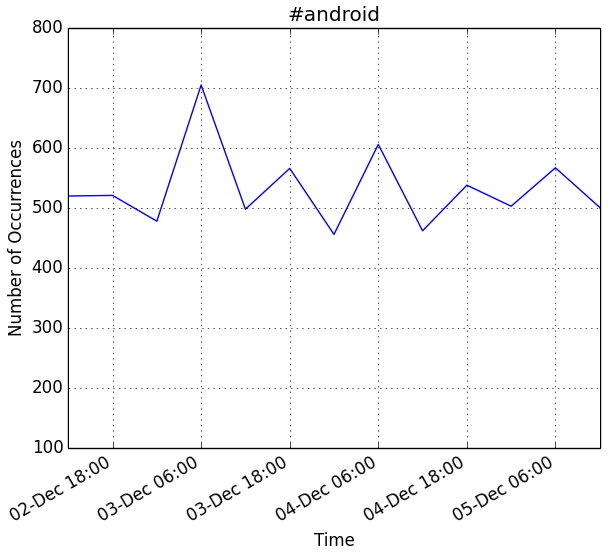
\includegraphics[width=0.45\textwidth]{android}
        \label{fig:android}
    }
    \subfigure[\#blackfriday]{
        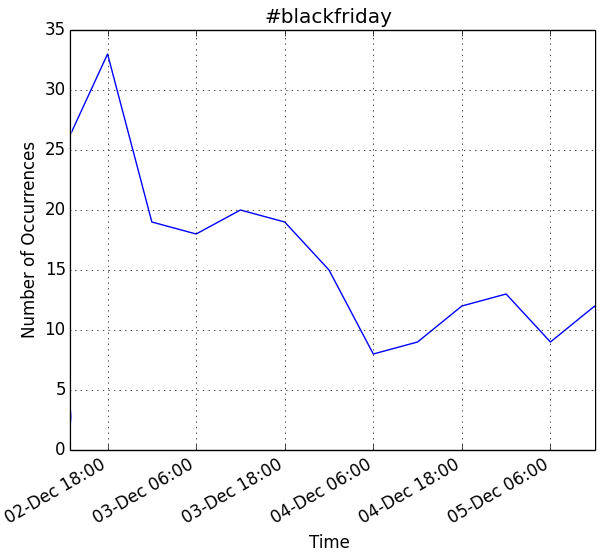
\includegraphics[width=0.45\textwidth]{blackfriday}
        \label{fig:blackfriday}
    }
    \caption{Usage of hashtags over the period that the dataset was collected.}
\end{figure}

\section{Project Goals}

The goal of this project is to develop an intelligent hashtag recommendation system for use with Twitter. For example, when a user writes a tweet such as: ``\emph{The golden gate bridge looks so nice today! I LOVE SF in this weather!}'', the system should recommend hashtags such as \texttt{\#SanFrancisco}, \texttt{\#California} or even \texttt{\#sohappy}, but should not recommend hashtags such as \texttt{\#ScienceFiction}, \texttt{\#amreading} or \texttt{\#fantasy}.

The objective is to make it easier for users to select appropriate meaningful hashtags for their tweets, and in doing so, begin to tackle the problems presented by the sheer quantity and redundancy of hashtags in Twitter. The aim is that the user will be able to see hashtag suggestions in real-time as they are typing a tweet, thus making them more likely to publish tweets with accurate hashtag data.

Such a recommendation system would also need to aid users in the navigational and exploratory aspects of folksonomies. For example, when a user performs a search on Twitter for the hashtag \texttt{\#BGT}, the system should display not only those tweets that contain \texttt{\#BGT}, but also tweets that are relevant to `Britain's Got Talent' but do not contain \texttt{\#BGT}.

Therefore, another objective for this project is to make it easier for users to navigate and search the content available on Twitter, thus making the fragmented hashtag data already published to Twitter easier to search and navigate. The aim is that the same recommendation system used to suggest hashtags for content a user is creating could also be applied to a search query to provide an expanded query that can then be used to query Twitter.

\pagebreak

\chapter{Background Literature \& Related Work}
\label{chap:litreview}
The main design goals behind hashtags are to categorise tweets and allow them to show up more easily in searches\footnote{\url{https://support.twitter.com/articles/49309-using-hashtags-on-twitter}}. Whilst the task that this project is aiming to complete is novel and fairly unexplored, it is well connected with other experiments, systems and projects within the research community.

\section{Traditional Recommendation Systems}
Traditional recommendation systems are in place all over the web today. From music discovery services \todo{Add screenshots of existing recommendation services?}(such as Last.fm\footnote{\url{www.last.fm}}) to suggested purchases on retail sites (like on the front page of Amazon\footnote{\url{www.amazon.co.uk}}), these systems are all personalised recommendation engines that take an individual user's preferences and use them to provide suggestions tailored to that user.

Most personalised recommendation systems employ a set of techniques known as collaborative filtering. These techniques were first coined by \textcite{Goldberg:1992}, where a system named \emph{Tapestry} was created that allowed people to attach annotations to documents, and then use that information to filter the documents for other users.

One common implementation of collaborative filtering is the so-called ``user-to-user'' approach. ``User-to-user'' collaborative filtering works by taking the preferences of a user $A$, and finding a small subset of other users in the system that have similar preferences. For each user $B$ in the subset, any items that $B$ has adopted that $A$ hasn't are added to a ranked list of suggestions. $A$ is now more likely to adopt items in the list than the items of another random person \parencite{Schafer:2001}.

Another approach to provide relevant recommendations to a user is the use of content-based recommendation systems. This is a type of system that recommends items relevant to other items by comparing the details and descriptions of the items themselves. This can be extended to suggest items for a user by comparing a content-based description of the user's preferences with the descriptions of the items \parencite{Pazzani:2007}.

A key issue with content-based filtering is that the recommendations can only be as accurate as the algorithm used to derive a user's profile. There are a number of algorithms available to build user profiles, depending upon the context, but essentially a content-based profile is created using a weighted vector of item features. The weights mark the importance of each feature to the user, and can be computed from individually rated content vectors.

\textcite{Cantador:2010} studied and evaluated a number of content-based recommendation models based upon the premise of user and item profiles being described in terms of weighted lists and tags. Through their experiments they found that models that focused on user profiles outperformed the models oriented towards item profiles in nearly every test. They go on to suggest that a better way of profiling users would be through the use of tag clustering.

Instead of limiting recommendation systems to the accuracy of their classifiers, a common approach is incorporate relevance feedback techniques. Relevance feedback is a process that was originally designed for information retrieval, and works on the assumption that a user can not always correctly encapsulate into a query what it is they are searching for. It works by allowing a user to create an initial query to which an initial set of results is returned. Out of these initial results, the user can then mark certain results as relevant or irrelevant, and this information is then submitted and used to refine the original query and return more relevant results to the user \parencite{Salton:1990}.

\textcite{Utiyama:2006} showed that it is possible to combine collaborative filtering, content-based filtering and relevance feedback techniques into one system to provide better recommendations.

\section{Assigning Labels with Machine-Learning Techniques}
Although there exists a long history of research into traditional recommendation algorithms, the data structure of a folksonomy is distinct from those found in traditional problems. This has led to a new generation of supervised learning classification algorithms which can be applied to the problem of assigning labels to resources.

In order to facilitate the comparison of resources, tags and users, aggregate projections of the data can be constructed. This reduces the dimensionality of the data by sacrificing some information \parencite{Schmitz:2006}. There are two main classes of algorithms that perform this task: feature \emph{selection}, which reduces the size of a dataset by selecting a subset of the data, and feature \emph{extraction}, which uses the existing data to generate entirely new features. Despite the improved results that feature extraction can provide, their computational cost and memory requirements can often make them impractical for use on the extremely large datasets common with Folksonomies \parencite{Gemmell:2009}.

One compromise to this trade-off is to use an algorithm such as Hebbian Deflation, which approximates the outputs of the intensive feature extraction techniques, but with lower computational cost and memory requirements \parencite{Oja:1985}. \textcite{Gemmell:2009} used this approach coupled with a \todo{Add more about K-Nearest Neighbour implementation?}K-Nearest Neighbour classifier to find appropriate tags for a given resource. This was done by finding `neighbouring' users: ``Neighbours are selected only if they have tagged the query resource and tags are selected for the recommendation set only if they have been applied by the neighbour to the resource.'' It was tested on data from the popular bookmarking site Delicious\footnote{\url{http://delicious.com/}} and from Citeulike\footnote{\url{http://www.citeulike.com/}}, a tool that enables researchers to manage and discover scholarly references, and it was found to be a successful approach with giving results.

\textcite{Niwa:2006} took a different approach to overcome the limitations of collaborative filtering. Using a modified version of the \todo{Add more TF-IDF implementation detail?}TF-IDF \parencite{Salton:1988}, they calculate the affinity level between users and tags (where affinity level is a measure of how frequently a user uses a particular tag), and then use this to calculate the similarity between tags. These similarity measures are then clustered using a custom clustering algorithm to provide a set of recommended tags for a given user and resource. This enabled them to adjust the level at which a user's preferences were taken into account when determining recommendations, as well as providing a simple solution to the tag redundancy issue found across most Folksonomies.

Another popular machine-learning approach to the folksonomy tag recommendation problem is the use of a \todo{Add more about Naive Bayes implementation?}Naive Bayes classifier. Naive Bayes has been an accepted tool in information retrieval for a long time, with some early literature dating back over 50 years \parencite{Maron:1960}, and has recently been seeing a renaissance within the machine-learning community.

As shown by \textcite{DePessemier:2010}, Naive Bayes can be easily adapted and extended to work in the context of providing recommendations to match a query or a set of user preferences. In particular, their algorithm relied upon the general user preferences for cases where the classifier produced an uncertain outcome, and became more context specific on a sliding scale as the classifer gave more certain probabilities.

\section{Approaches to Hashtag Recommendation}
Even though providing hashtag recommendations and suggestions is still a new and largely unexplored field, there have been several efforts to improve the hashtag experience for Twitter users.

The current hashtag system on Twitter (\autoref{fig:twittersuggest}) uses a non-personalised auto-complete tool to provide suggestions to the user. Whenever a hash symbol (\#) is typed in the tweet composer, the system simply suggests hashtags starting with the letters that the user has typed so far. These suggestions are chosen from a tiny subset of hashtags, taken from a mixture of those currently trending\footnote{Trending hashtags are those with the highest rise in usage within a given time period.} and from the user's history. Whilst better than not having suggestions at all, this system is only truly useful in one of two specific use cases: when the user knows the starting letters of a trending hashtag they want to use, or are trying to recall a hashtag that they have previously used. This system does not help the user choose the correct hashtag for the content of their tweet.

\begin{figure}[htpb]
    \centering
    
\includegraphics[width=0.5\textwidth]{twittersuggest.png}
    \caption{Twitter's current hashtag suggestion system.\label{fig:twittersuggest}}
\end{figure}

By assuming that the primary purpose of hashtags is to categorise tweets and improve searching (as Twitter envisioned), \textcite{Zangerle:2011} created a system that recommends hashtags for a tweet by taking hashtags from other tweets that are textually similar to the query. The similarity between tweets is calculated with the TF-IDF model. The hashtags are then extracted from the similar tweets, ranked according to how similar the tweets were to the original query, and returned as a list of suggestions to the user. A number of different ranking algorithms were tested, but this was found to be the most successful.

After studying the advantages of providing personalised recommendations in retail situations on a per-user basis, \textcite{Kywe:2012} realised that a similar approach towards hashtags could prove fruitful. Hashtag use varies from user to user, with some users using the latest trending hashtags, other users only using a specific set or type of tag, and with some users barely using them at all. They proposed a personalised hashtag recommendation system that considers both user preferences and the query tweet content: the system creates a ranked list of hashtags from both the most similar users and most similar tweets. This gave promising results, although it was noted that this may not be the best recommendation system for all types of tweets and hashtags.

\textcite{Shepitsen:2008} used a hierarchical agglomerative clustering algorithm to profile users and provide personalised recommendations in collaborative tagging systems. They found that clusters of tags can be effectively used to ascertain a user's interests, which could then be used in a traditional content-based recommendation approach. This technique worked well, particularly for dense folksonomies such as Last.fm.

Observers of social media have realised that hashtags play a dual role within the online microblogging communities, such as Twitter. On one hand, hashtags fulfil the design goals that Twitter created them to accomplish (bookmarking and improving search); on the other hand, however, they serve as a badge of community membership: connecting users together. \textcite{Yang:2012} took this duality into account when attempting to create a hashtag recommendation system by training a SVM (support vector machine) classifier with a variety of features taken from the tweet metadata to overcome the duality and suggest relevant hashtags.

\pagebreak

\chapter{Analysis}
\label{chap:analysis}

As previously discussed in Chapter~\ref{chap:introduction}, there is a need for a hashtag recommendation system to improve the quality and clarity of hashtags in Twitter, as well as to aid navigation of the already existing fragmented data. This leads to the two main requirements the system in this project must fulfil:
\begin{itemize}
    \item Users should be able to compose and publish tweets whilst suggesting hashtags relevant to the content of their tweets.
    \item Users should be able to search for a hashtag and view related tweets, including those that don't contain that hashtag.
\end{itemize}

As seen from the research and discussion presented in Chapter~\ref{chap:litreview}, most existing approaches to providing recommendations within a folksonomy make extensive use of user preferences in their algorithms. From calculating a `neighbourhood' of similar users to falling back on a set of users' preferences when the data is unclear, most current approaches provide a personalised recommendation system.

This raises the question of whether hashtags are clearly defined, or whether their meanings (and therefore the tweets they apply to) are dependent upon user opinion. Through the preliminary examination of a sample Twitter dataset conducted in Chapter~\ref{chap:introduction}, this project is inclined to believe that the correct usage of a hashtag is independent of how frequently a particular user uses that hashtag. Indeed, it could be argued that it is this preference of users to use a particular hashtag that results in users incorrectly using hashtags in the first place --- which is the very problem this project is aiming to tackle.

This indicates another requirement of the recommendation system:
\begin{itemize}
    \item The system must provide identical recommendations for all users; user preferences should not be taken into account.
\end{itemize}

As with all folksonomies, there is not a predefined set of hashtags available to users on Twitter, meaning new hashtags are created and used every day. With this in mind it becomes clear that a lot of data will be needed to train the recommendation system, so that it successfully recognises and recommends a sufficient number of hashtags. This gives another requirement of the system:
\begin{itemize}
    \item The system must be capable of training on a sufficiently large dataset of tweets, with potential to use the live data from the Twitter stream.
\end{itemize}

Lastly, Twitter is available through its web platform on practically every internet-connected device that exists today. For this system to be successfully implemented and used by Twitter users, it too must be available on all of Twitters supported devices. In addition to this, it must be as easy to post a tweet using the recommendation system as it is on Twitter.
\begin{itemize}
    \item The system must be accessible through a web interface that provides quick and easy access to the recommendation system.
\end{itemize}

\section{Requirements}
From the broad requirements outlined above, a set of formal requirements can be inferred:

\subsection{Functional Requirements}
\begin{enumerate}
    \item \label{func:publish} The system must allow the user to log in and publish tweets using their Twitter account.
    \item \label{func:suggest} The system must provide hashtag recommendations as the user is writing a tweet.
    \item \label{func:search} The system must perform a hashtag search through a large dataset of tweets and return all relevant tweets, including those that do not contain the search query.
    \item \label{func:genmodel} The system must use information from a large dataset of tweets to generate a model representing each hashtag.
    \item \label{func:notpersonal} The system must only use the data available through the Twitter API, and not make use of any other externally collected metrics, such as user preferences.
    \item \label{func:compmodels} The system must be able to compare tweets against its representational hashtag models.
    \item \label{func:stream} \emph{Optional:} In place of a large dataset, the system must be able to use information from the live Twitter stream.
    \item \label{func:probabilities} \emph{Optional:} The system must provide probabilities for how likely a hashtag is to be related to a tweet.
\end{enumerate}

\subsection{Non-Functional Requirements}
\begin{enumerate}
    \item \label{nfunc:web} The system must be accessible via a web interface.
    \item \label{nfunc:easy} The system must be responsive and easy to use.
    \item \label{nfunc:qsearch} The system must be able to perform searches quickly.
    \item \label{nfunc:qsuggest} The system must be able to make hashtag recommendations quickly.
    \item \label{nfunc:graphs} \emph{Optional:} The system must be able to produce visualisations to provide an easy way to interpret the hashtag recommendations/assignments.
    \item \label{nfunc:mobile} \emph{Optional:} The system must be accessible via mobile web browsers.
\end{enumerate}

\pagebreak

\chapter{Design}
\label{chap:design}

\section{Architecture}

The primary aim of the system is to produce an ordered list of recommended hashtags for a given string with a maximum length of 140 characters (a tweet). The secondary aim is to facilitate query expansion when searching Twitter for a hashtag. Due to non-functional requirement~\ref{nfunc:web}, both of these sub-systems must be available through a web interface. It is unreasonable and infeasible to expect all necessary training and classification to occur in code running within the user's browser, especially considering that some of those browsers might be on low-powered mobile platforms. For these reasons, a client-server architecture (\autoref{fig:clientserver}) has been chosen for the system.

\begin{figure}[htpb]
    \centering
    \begin{tikzpicture}
        \node[draw,rectangle,minimum width=2cm,minimum height=1.5cm] (server) at (0:0) {Server};
        \node[draw,circle] (a) at +(0:2.5) {Client};
        \node[draw,circle] (b) at +(72:2.5) {Client};
        \node[draw,circle] (c) at +(2*72:2.5) {Client};
        \node[draw,circle] (d) at +(3*72:2.5) {Client};
        \node[draw,circle] (e) at +(4*72:2.5) {Client};
        \foreach \from in {a, b, c, d, e}
        \draw [->,thick] (\from) -- (server);
    \end{tikzpicture}
    \caption{A simplified diagram of the client-server architecture.}
    \label{fig:clientserver}
\end{figure}

Using a client-server software model will allow for a distinct separation between the hashtag recommendation system and any interfaces that make use of the tool. The server (Figure~\ref{fig:serveroverview}) will be running a single instance of the recommendation engine, and will handle all training and classification events. Multiple clients (Figure~\ref{fig:clientoverview}) can then query the classifier running on the server for either hashtag suggestions or a search query expansion.

\begin{figure}[htpb]
    \centering
    \subfigure{
        \begin{tikzpicture}
            \node[rectangle,draw,text width=5cm,anchor=north,rectangle split, rectangle split parts=2,text justified] (server) {
                \textbf{Server}
                \nodepart{second}- Hashtag recommendation\newline
                - Search query expansion\newline
                - Training classifier\newline
                - Persistent state
            };
        \end{tikzpicture}
        \label{fig:serveroverview}
    }
    \subfigure{
        \begin{tikzpicture}
            \node[rectangle,draw,text width=5cm,anchor=north,rectangle split, rectangle split parts=2,text justified] (client) {
                \textbf{Client}
                \nodepart{second}- Twitter authentication\newline
                - Twitter API calls\newline
                - Send requests to server\newline
                - Receive data from server
            };
        \end{tikzpicture}
        \label{fig:clientoverview}
    }
    \caption{Functional overviews of the server and client.}
\end{figure}

This design ensures that there is a very light load on the clients using the tool, which is an ideal solution to enabling usage of the system from all internet-connected devices (non-functional requirements \ref{nfunc:web} and \ref{nfunc:mobile}).

Another benefit of using a centralised server to encapsulate the hashtag recommendation system is the clear separation of functionality between the client and server. This means that the interface that the user sees and interacts with is distinct from the technical functionality --- enabling multiple differently styled interfaces to connect to the recommendation server. It even presents the possibility to one day integrate easily with the Twitter web platform itself.

\section{Abstract Implementation}

When using a client-server execution model, it is important to correctly balance the tasks that need to be executed between the clients, the server and the users. Placing a high computational load on the users' machines can limit the accessibility of the system, whilst placing a high computational load on the server can cause a slow-down or even interrupted service for all clients using the system.

The server encapsulates the hashtag classifier system. It will have the ability to train the classifier on tweet data independently and asynchronously to the other tasks that the classifier may need to perform. The training will perform as many of the computationally intensive operations on the classifier model as it feasibly can, to ensure that any requests from a client to classify a tweet or expand a query are performed as quickly as possible (fulfilling non-functional requirements \ref{nfunc:qsearch} and \ref{nfunc:qsuggest}). Asynchronous training will also provide the opportunity to integrate training data from the live Twitter stream (as described in functional requirement~\ref{func:stream}).

The client's primary focus will be delivering the interface to the users. It will provide a way for the user to interact with the recommendations and search tools available on the server, as well as handling the users' authentication with Twitter and calling appropriate tweet/search functions in the Twitter API.

\todo{Make this diagram neater}
\begin{figure}[htpb]
    \centering
    \begin{tikzpicture}[
        node distance=7mm,
        title/.style={anchor=west,font=\fontsize{9}{9}\color{black}\ttfamily},
        typetag/.style={rectangle, draw=black!50, anchor=west}
    ]
        % Server
        \node (server) [title] {Server};
            \node (classifier) at ($(server.west)+(0,-28pt)$) [title,xshift=2mm] {Classifier};
                \node (worker) at ($(classifier.west)+(0,-28pt)$) [title,xshift=2mm] {Worker Process};
                    \node (train) [below=of worker.west,typetag] {Training Function};
                \node (swebserver) at ($(train.west)+(0,-32pt)$) [title] {Web Server};
                    \node (recommend) [below=of swebserver.west,typetag] {Hashtag Recommendation};
                    \node (query) [below=of recommend.west,typetag] {Search Query Expansion};

        \node (workerbox) [draw,fit={(worker) (train)}] {};
        \node (swebserverbox) [draw,fit={(swebserver) (recommend) (query)}] {};
        \node (classifierbox) [draw,fit={(classifier) (workerbox) (swebserverbox)}] {};
        \node (serverbox) [draw,fit={(server) (classifierbox)},line width=1.5pt] {};


        % Client
        \node (client) at (7.5cm, 0) [title] {Client};
        \node (cwebserver) at ($(client.west)+(0,-28pt)$) [title,xshift=2mm] {Web Server};
                \node (auth) [below=of cwebserver.west,typetag] {Twitter Authentication};
                \node (api) [below=of auth.west,typetag] {Twitter API Calls};
                \node (interface) [below=of api.west, typetag] {Interface};

        \node (cwebserverbox) [draw,fit={(cwebserver) (auth) (api) (interface)}] {};
        \node (clientbox) [draw,fit={(client) (cwebserverbox)},line width=1.5pt] {};


        % Users
        \node (a) at (8.3cm, -5.3cm) [draw,circle,minimum width=1cm] {User};
        \node (b) at (9.8cm, -5.3cm) [draw,circle,minimum width=1cm] {User};
        \node (c) at (11.3cm, -5.3cm) [draw,circle,minimum width=1cm] {User};


        % Twitter
        \node (twitter) at (6.4cm, 2.5cm) [cloud,draw,cloud puffs=10,cloud puff arc=120,aspect=2,inner ysep=1em] {Twitter};


        % Arrows
        \draw[<->] (a) -- (interface);
        \draw[<->] (b) -- (interface);
        \draw[<->] (c) -- (interface);
        \path[<->] (clientbox) edge node[sloped, anchor=center, above] {\footnotesize HTTP} (swebserverbox);
        \draw[<->] (clientbox) -- (twitter);
        \draw[->,dashed] (twitter) -- (train);
    \end{tikzpicture}
    \caption{An abstract view of the implementation of the system.}
    \label{fig:abstractdetail}
\end{figure}

\section{User Interface}
Whilst the primary focus of this project is the creation of the tool to provide hashtag suggestions and query expansions (the server), a simple prototype interface will also be developed. This interface will remain simple, but will enable users to log in to Twitter, post tweets using hashtag suggestions, and search Twitter using query expansion.

Figure~\autoref{fig:wireframe:tweet} shows the design of the interface for creating a tweet. It follows conventional HCI principles, including displaying the site name and navigation in the top left, and having the user's username and user-oriented controls in the top right. There is a single box for the user to type their tweet message into, and as they are typing into this box, relevant hashtag suggestions will appear underneath. Clicking on one of these hashtags will insert it at the end of the text in the box.

Figure~\autoref{fig:wireframe:searchresults} shows the design of the interface for searching Twitter. It follows the same HCI guidelines as most other search results pages, and keeps the same layout as the tweet composition page (and indeed, all other pages in the client interface).

\begin{figure}[htpb]
    \centering
    \subfigure[Tweet composition page.]{
        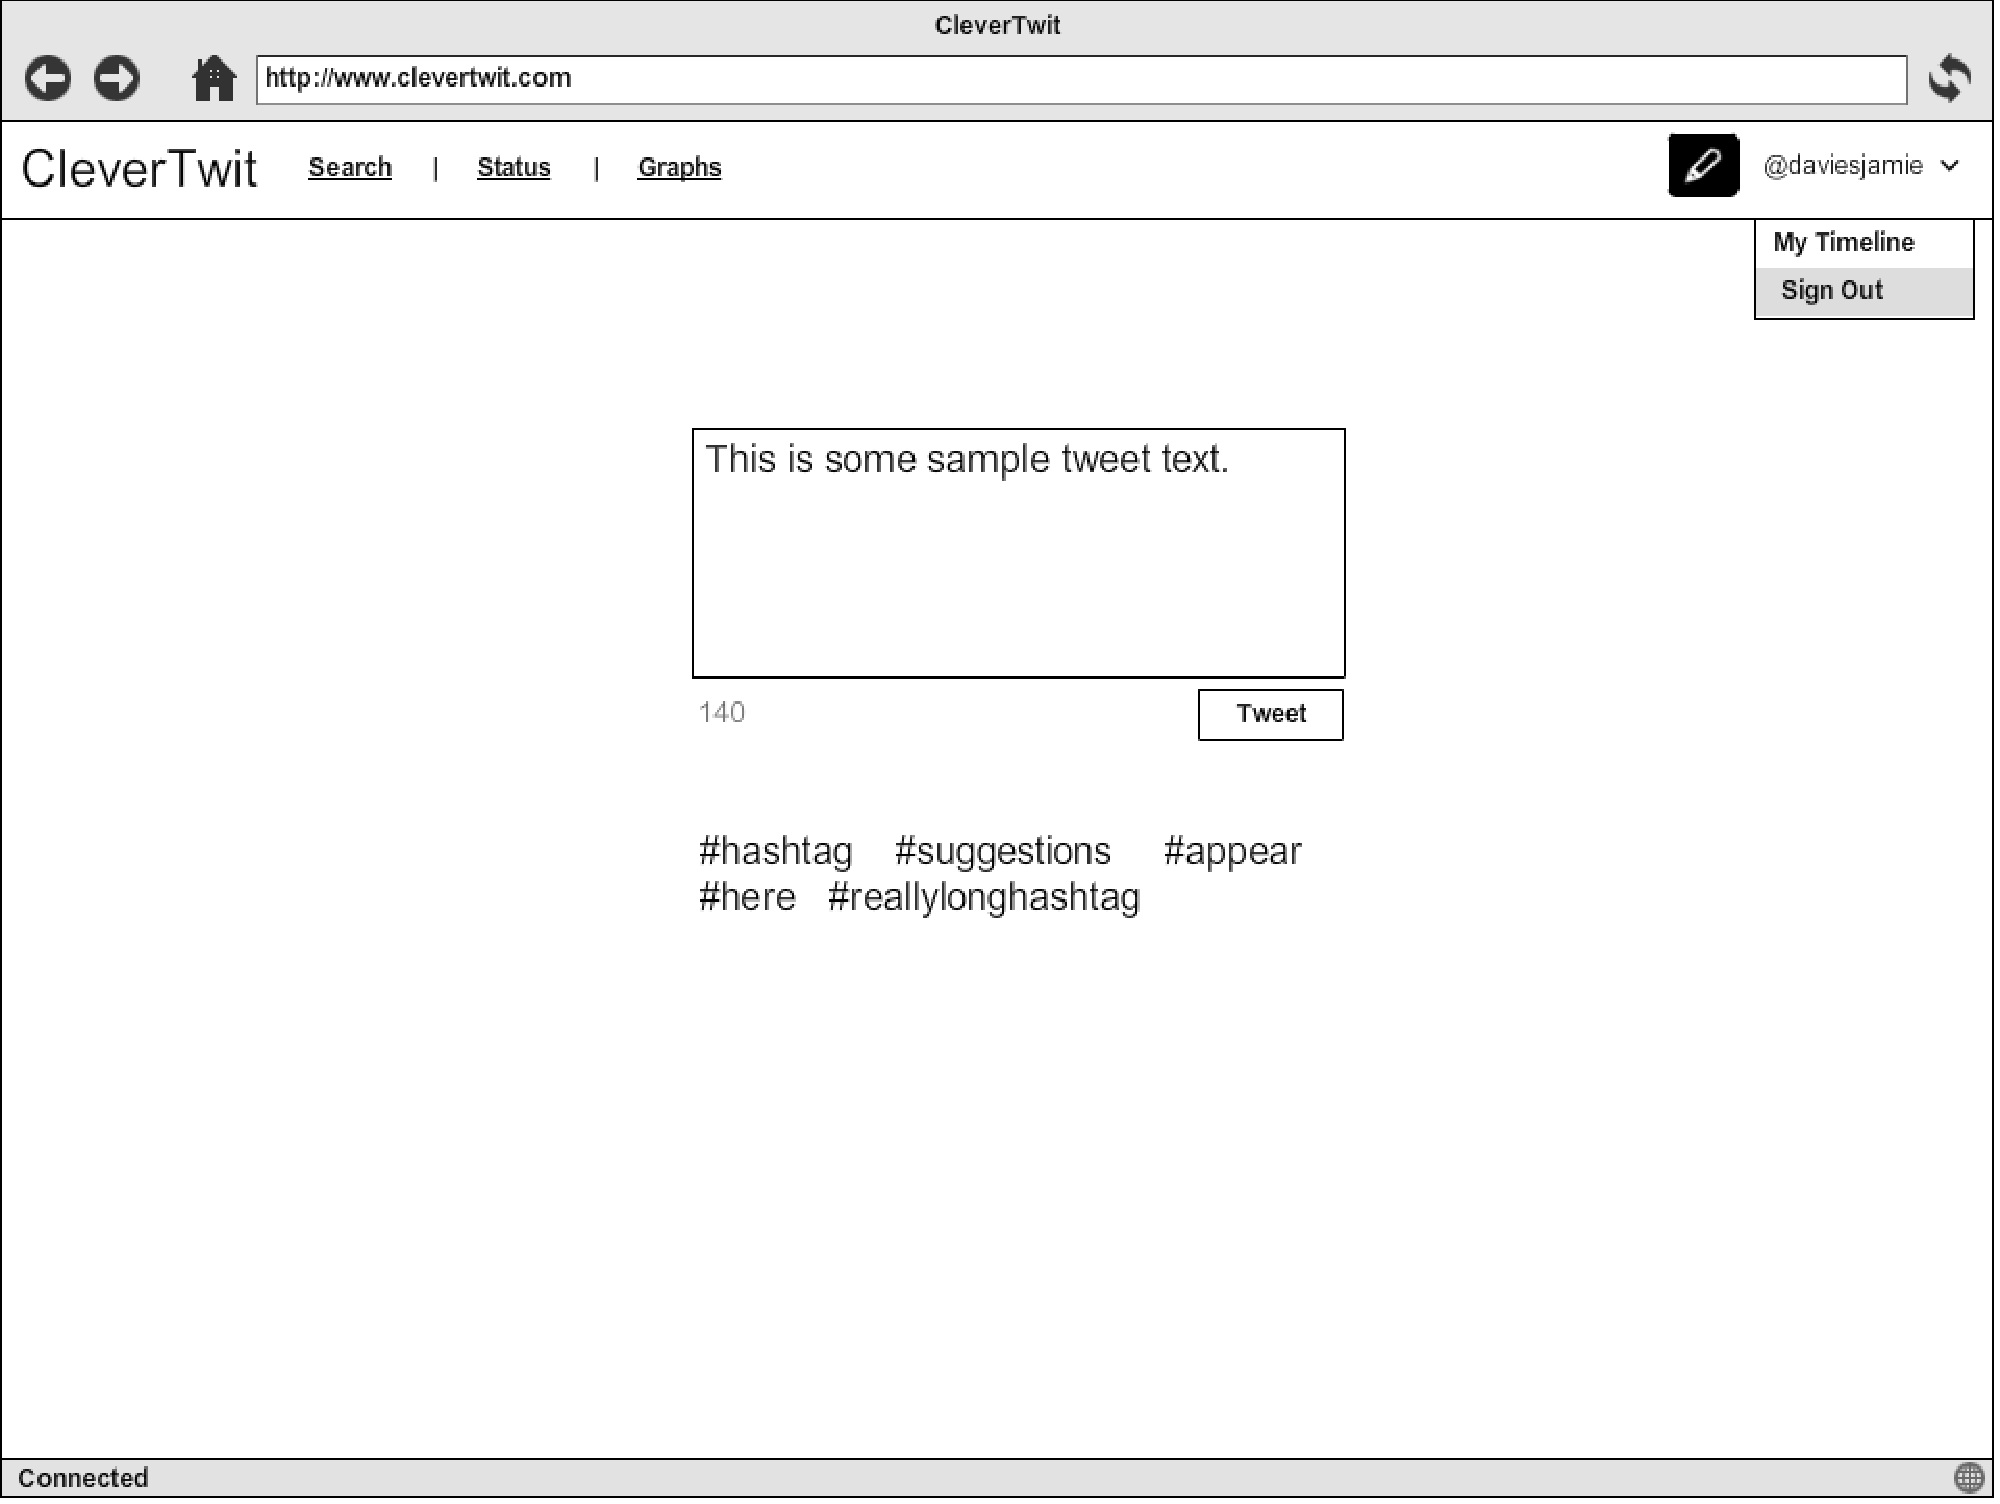
\includegraphics[width=0.9\linewidth]{wireframes/tweet.pdf}
        \label{fig:wireframe:tweet}
    }
%    \subfigure[The beginning search page.]{
%        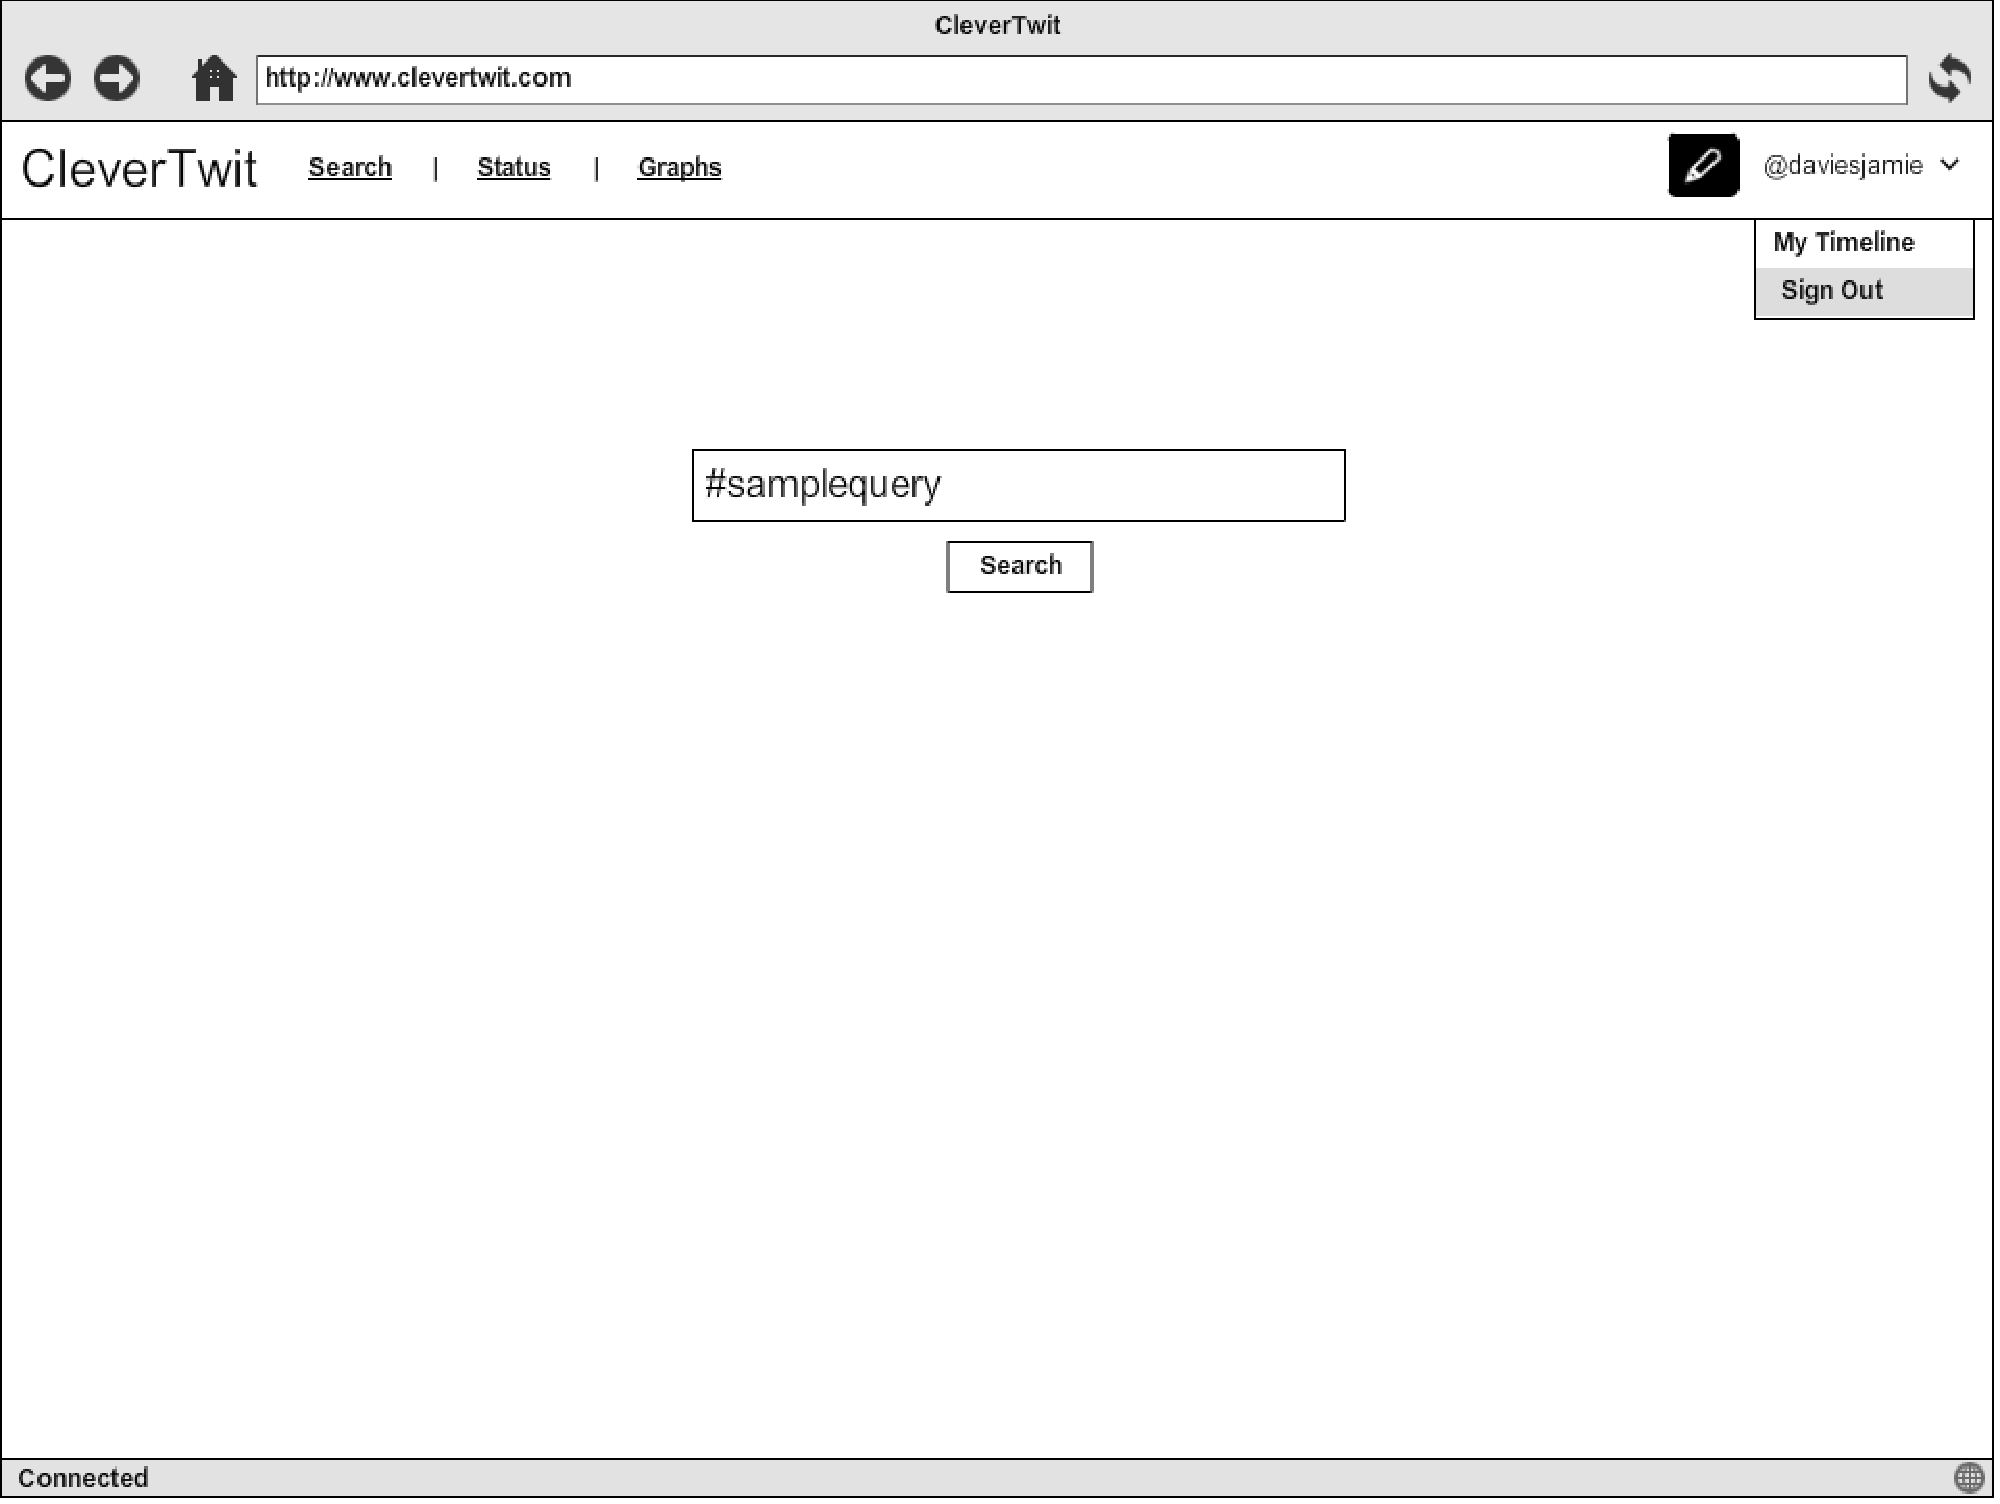
\includegraphics[width=0.8\linewidth]{wireframes/search.pdf}
%        \label{fig:wireframe:search}
%    }
    \subfigure[The search results page.]{
        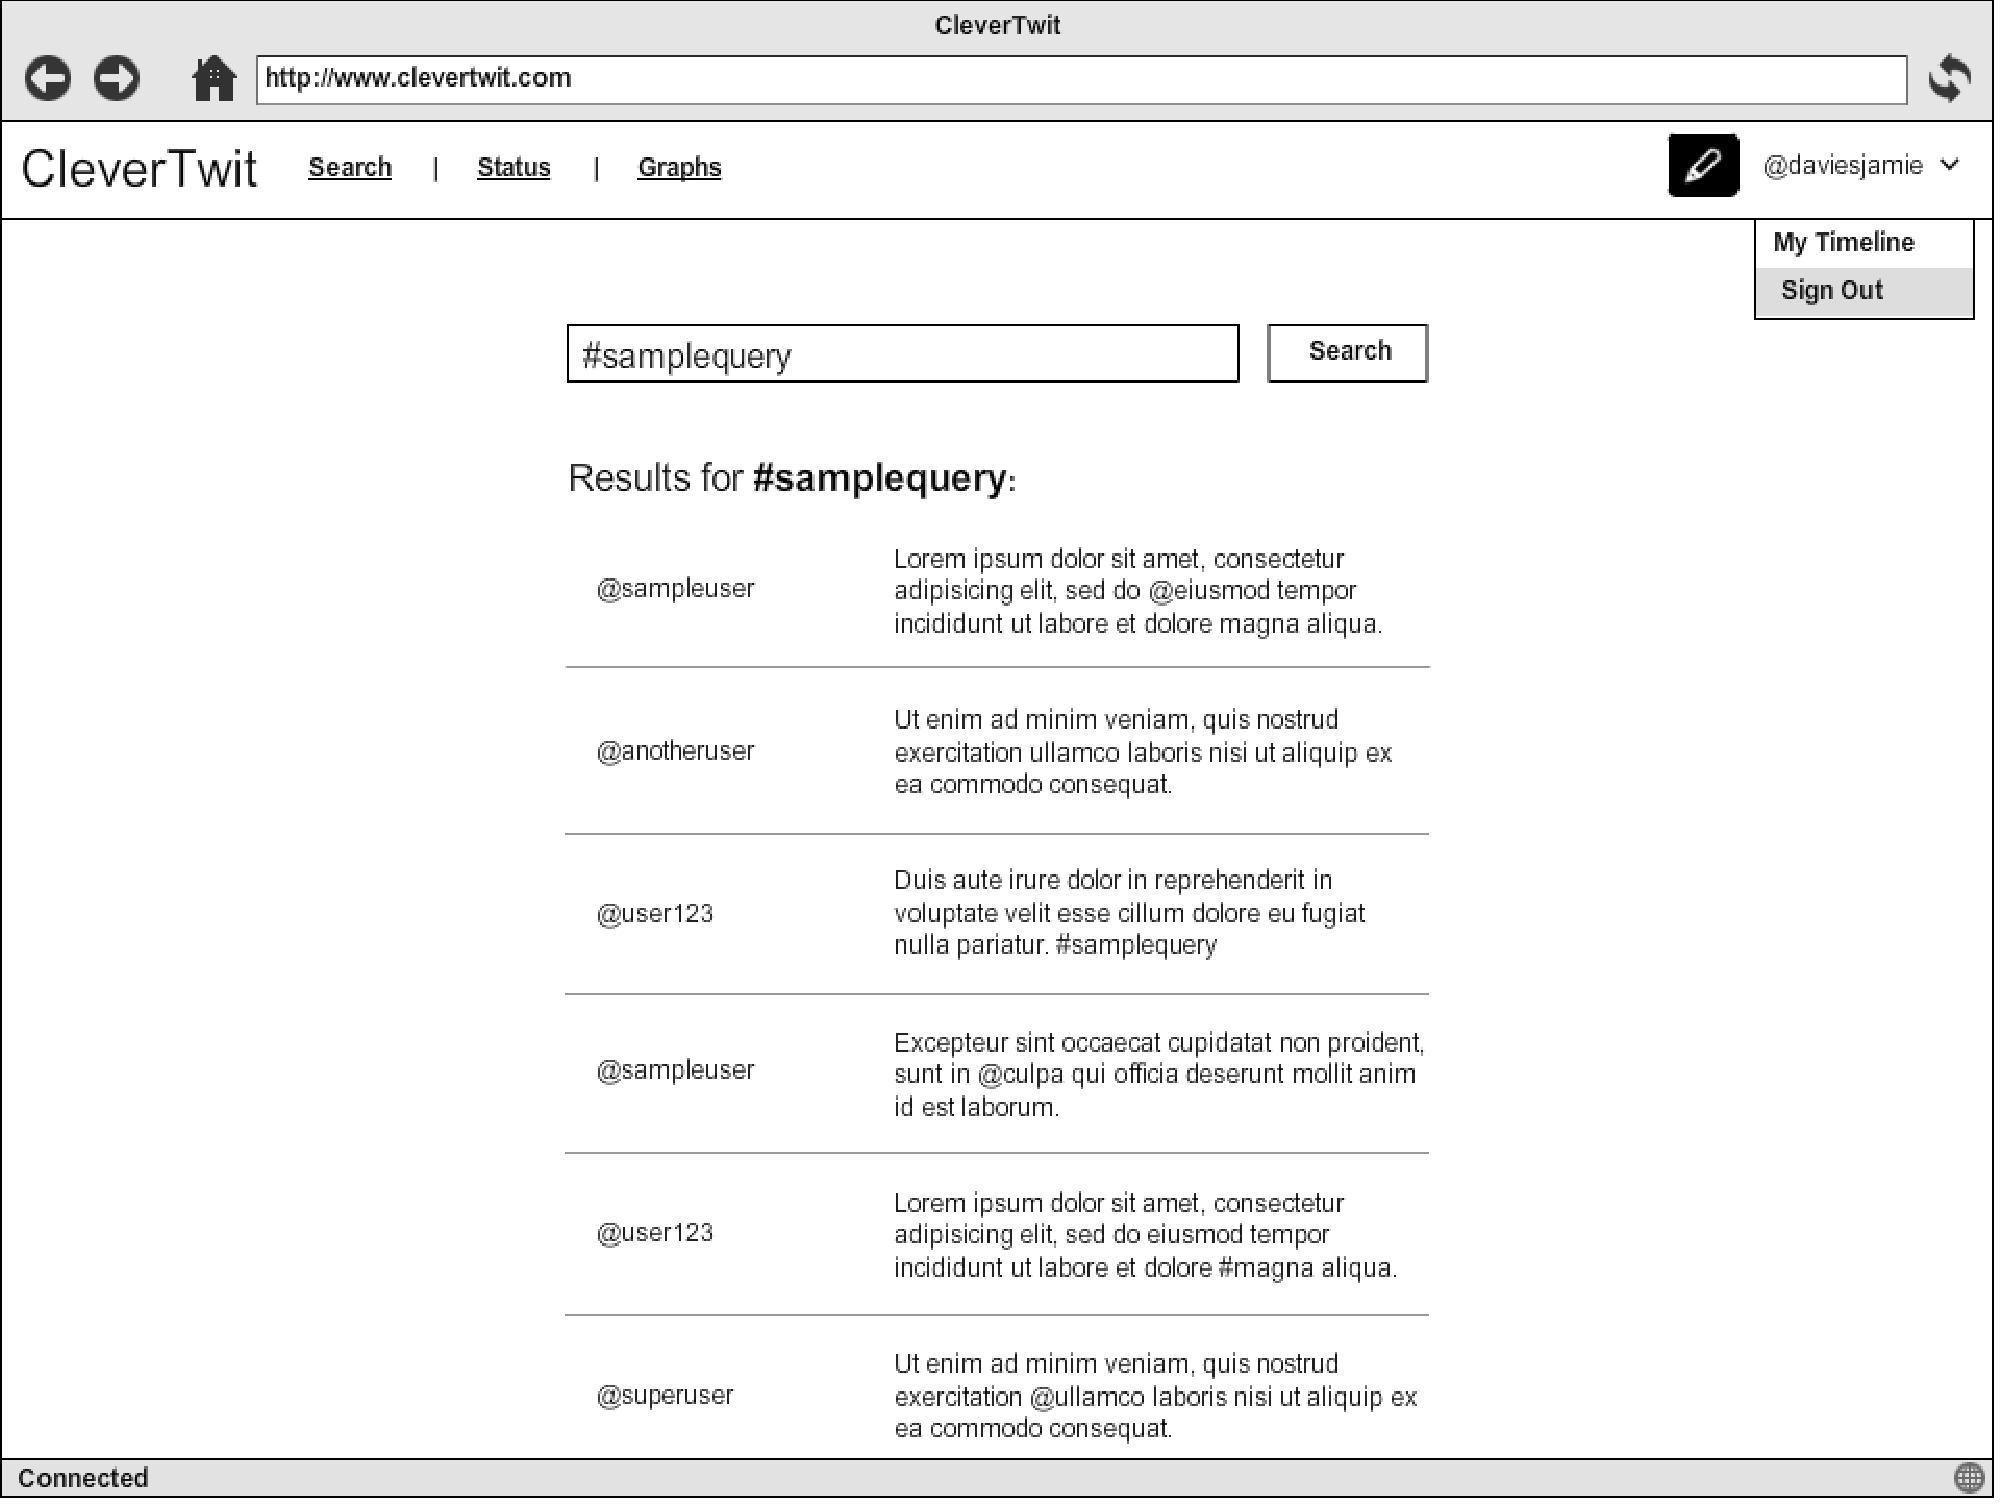
\includegraphics[width=0.9\linewidth]{wireframes/searchresults.pdf}
        \label{fig:wireframe:searchresults}
    }
    \caption{Wireframe designs of the prototype interface.}
    \label{fig:wireframes}
\end{figure}

\pagebreak

\chapter{Implementation}
\label{chap:implementation}

This chapter aims to explain how the system was implemented, and the decisions that were made during the implementation process. It will also explain any difficulties that were encountered, and how they were dealt with.

\section{Tools \& Technologies}
The first decision to make when implementing the system was to decide upon the programming languages, technologies and libraries that would be used.

Python 2.7 was chosen as the language of choice for the majority of the project, including both the server and the content management system for the client. Python is a widely used high-level programming language whose syntax emphasises code readability and maintainability. Most importantly, it has a strong developer community behind it, resulting in a large collection of excellent third-party libraries, including the following:

\begin{itemize}
    \item Django\footnote{\url{www.djangoproject.com}} offers a simple and flexible way of following the traditional MVC (Model-View-Controller) programming paradigm. This made it easy to develop the client system, by providing a structured way to keep the authentication and page generation separate from the layout and design of the page. Django also offers a pleasant interface to handling web requests.
    \item Flask\footnote{\url{http://flask.pocoo.org}} and Tornado\footnote{\url{www.tornadoweb.org}} are a web application frameworks made with Python, that make it simple to create efficient and scalable web APIs and WSGI applications. They are used to create and handle the HTTP endpoints for the server.
    \item Twython\footnote{\url{http://github.com/ryanmcgrath/twython}}, a thin but functional Python wrapper around the Twitter API, making Twitter API calls easily available within Python. It also provides a set of methods that handle OAuth authentication with Twitter.
\end{itemize}

Python 3 was not chosen for the project as it is still in its infancy. Many existing libraries written for Python have not yet been adapted for Python 3, and most operating systems or installers default to Python 2.7. To be successful, the system in this project has to be as easy to integrate and set up as possible --- and therefore Python 2.7 was chosen.

The client interface itself was written with a combination of HTML, CSS and Javascript. In particular, the following tools and libraries were used:

\begin{itemize}
    \item Twitter Bootstrap\footnote{\url{http://getbootstrap.com}}, a front-end framework that enables sleek and interactive interfaces with minimal customisation, allowing for easier and faster web development. It also has the bonus of being the UI toolkit that Twitter itself uses, and gives the client interface a look and feel similar to that of Twitter. Lastly, Bootstrap makes use of CSS3 to provide a full responsive interface, allowing the same web page to be viewed across all devices, regardless of the screen size --- which helps to fulfil non-functional requirement \ref{nfunc:mobile}.
    \item JQuery\footnote{\url{www.jquery.com}}, a Javascript library that contains a huge set of predefined functions and classes. It is designed to simplify client-side Javascript, and makes it much easier to manipulate the DOM from within Javascript --- it is used specifically within the client to perform AJAX requests to the server, and provide live hashtag suggestions.
\end{itemize}

Nginx\footnote{\url{www.nginx.org}} was used to proxy the requests to the client and server, as well as serving all static files. This not only significantly boosted the performance of the system, but it also made secure and accessible.

\section{Spout: A Data Stream Processing Framework}
To give the possibility of using either the live Twitter stream or a static file of tweets as the data source for the classifier, it was decided that the input data should be operated on as a stream. Doing so would allow identical processing of the tweet data, regardless of where the data came from.

A library with a fluent interface was created to enable such a processing paradigm. A fluent interface is the use of chaining method calls together to relay the instruction context of a subsequent call, to improve the readability of the code. At the heart of the library is the concept of a stream, which is simply a sequential (and not necessarily finite) collection of data items. The \verb+Stream+ class defines the basic operations that can be performed upon a data stream:

\begin{description}
    \item[Mapping] \hfill \\
        The items in one stream can be mapped to another stream. This is done by applying a supplied \verb+Function+ object to each item in the input stream, to produce another output stream.
        \mint{python}+stream.map(Function)+
    \item[Filtering] \hfill \\
        The items in a stream can be filtered, so that the resultant stream only contains items that match a given criteria. This is done by using a supplied \verb+Predicate+ to test each item in the input stream, and copies it to the output stream if it passes the test criteria.
        \mint{python}+stream.filter(Predicate)+
    \item[Processing (Consuming)] \hfill \\
        The items in a stream are used in some calculations or functionality that provides no further output to the stream. This is done by applying the supplied \verb+Operation+ to each item in the stream.
        \mint{python}+stream.for_each(Operation)+
\end{description}

The source of the stream could be easily changed from the live Twitter Stream to a JSON file, or even to a plain text file. The interface is highly customisable, allowing for custom stream implementations to be created --- all that is required is for the stream to sequentially output items of data.

The creation of this programming interface enabled a tweet processing pipeline to be constructed. The use of Spout has reduced the complexity of the pipeline, and makes the code much more readable, as seen in the code snippet in Listing~\ref{lst:trainingstream} taken from the training code for the classifier.

\begin{listing}[H]
    \begin{minted}[frame=lines,framesep=2mm]{python}
twitter = TweetStream(QueueBufferedQueue(3)))
twiter.connect()

twitter \
    .filter(TweetsWithHashtagsPredicate()) \
    .filter(TweetsInEnglishPredicate()) \
    .filter(NoRetweetsPredicate()) \
    .map(TokeniseTweetFunction()) \
    .for_each(TrainOperation(classifier)
    \end{minted}
    \caption{Code snippet demonstrating classifier training using Spout stream processing.}
    \label{lst:trainingstream}
\end{listing}

Another feature built into Spout that can be seen in Listing~\ref{lst:trainingstream} is the use of a \verb+BufferedQueue+ object when creating the data stream. Processing data from a live data source can present an infamous problem: the consumer-producer problem. This is where the input data source (in this case, the live Twitter stream) produces data faster than the system can process it, or vice-versa. Spout's \verb+BufferedQueue+ object defines a thread-safe queue object of an arbitrary size that when full, drops any extra items and ignores them. Similarly, if the queue is empty and another item is requested, the queue blocks the process asking for an item until another item is available. Thus, a trivial solution to the consumer-producer problem is presented, by filtering the input data source through a \verb+BufferedQueue+ before processing it.

\subsection{Publication}

Spout has been developed in an abstract, isolated fashion, meaning that it is distinct from the hashtag suggestion system presented in this project. This means that Spout could be useful in a number of scenarios other than Twitter processing. Because of this, Spout has been made available independently from this project. The full source for Spout is available on GitHub\footnote{\url{http://github.com/daviesjamie/spout}}.

In addition to open-sourcing Spout, it has also been made available on the Python Package Index (PyPI)\footnote{\url{https://pypi.python.org/pypi/spout/0.1.5}}. This has been a huge success, with approximately 3000 recorded downloads at the time of writing.

\todo[inline]{Classifier/Bayes}
\todo[inline]{Client}

\pagebreak

\chapter{Testing}
\label{chap:testing}
\todo[inline]{Testing section.}

\pagebreak

\chapter{Conclusion}
\label{chap:conclusion}
\todo[inline]{Conclusion section.}

\pagebreak

\begin{appendices}
\chapter{Time Management}

\begin{landscape}
    \label{appendix:gantt}
    This is a Gantt chart showing the scheduled progression through the different aspects of the project.

    \begin{figure}[H]
        \centering
        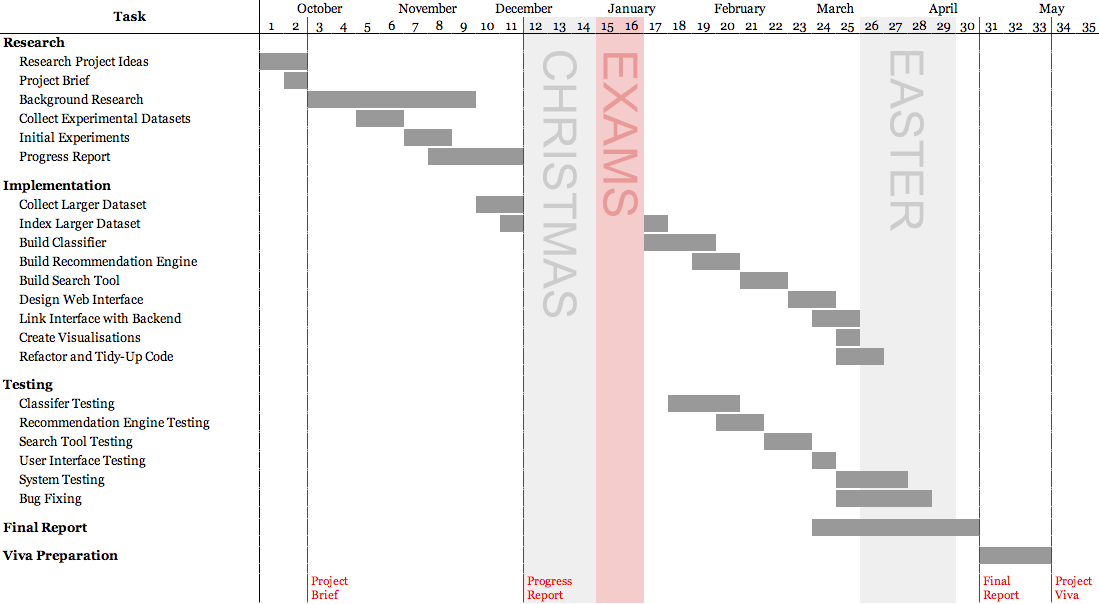
\includegraphics[height=0.85\textwidth]{gantt.png}
    \end{figure}
\end{landscape}

\chapter{Testing Plans \& Results}
\pagebreak

\chapter{REST API Interface}
\pagebreak

\chapter{Original Project Brief}
\vspace*{-3cm}
\hspace*{-2.4cm}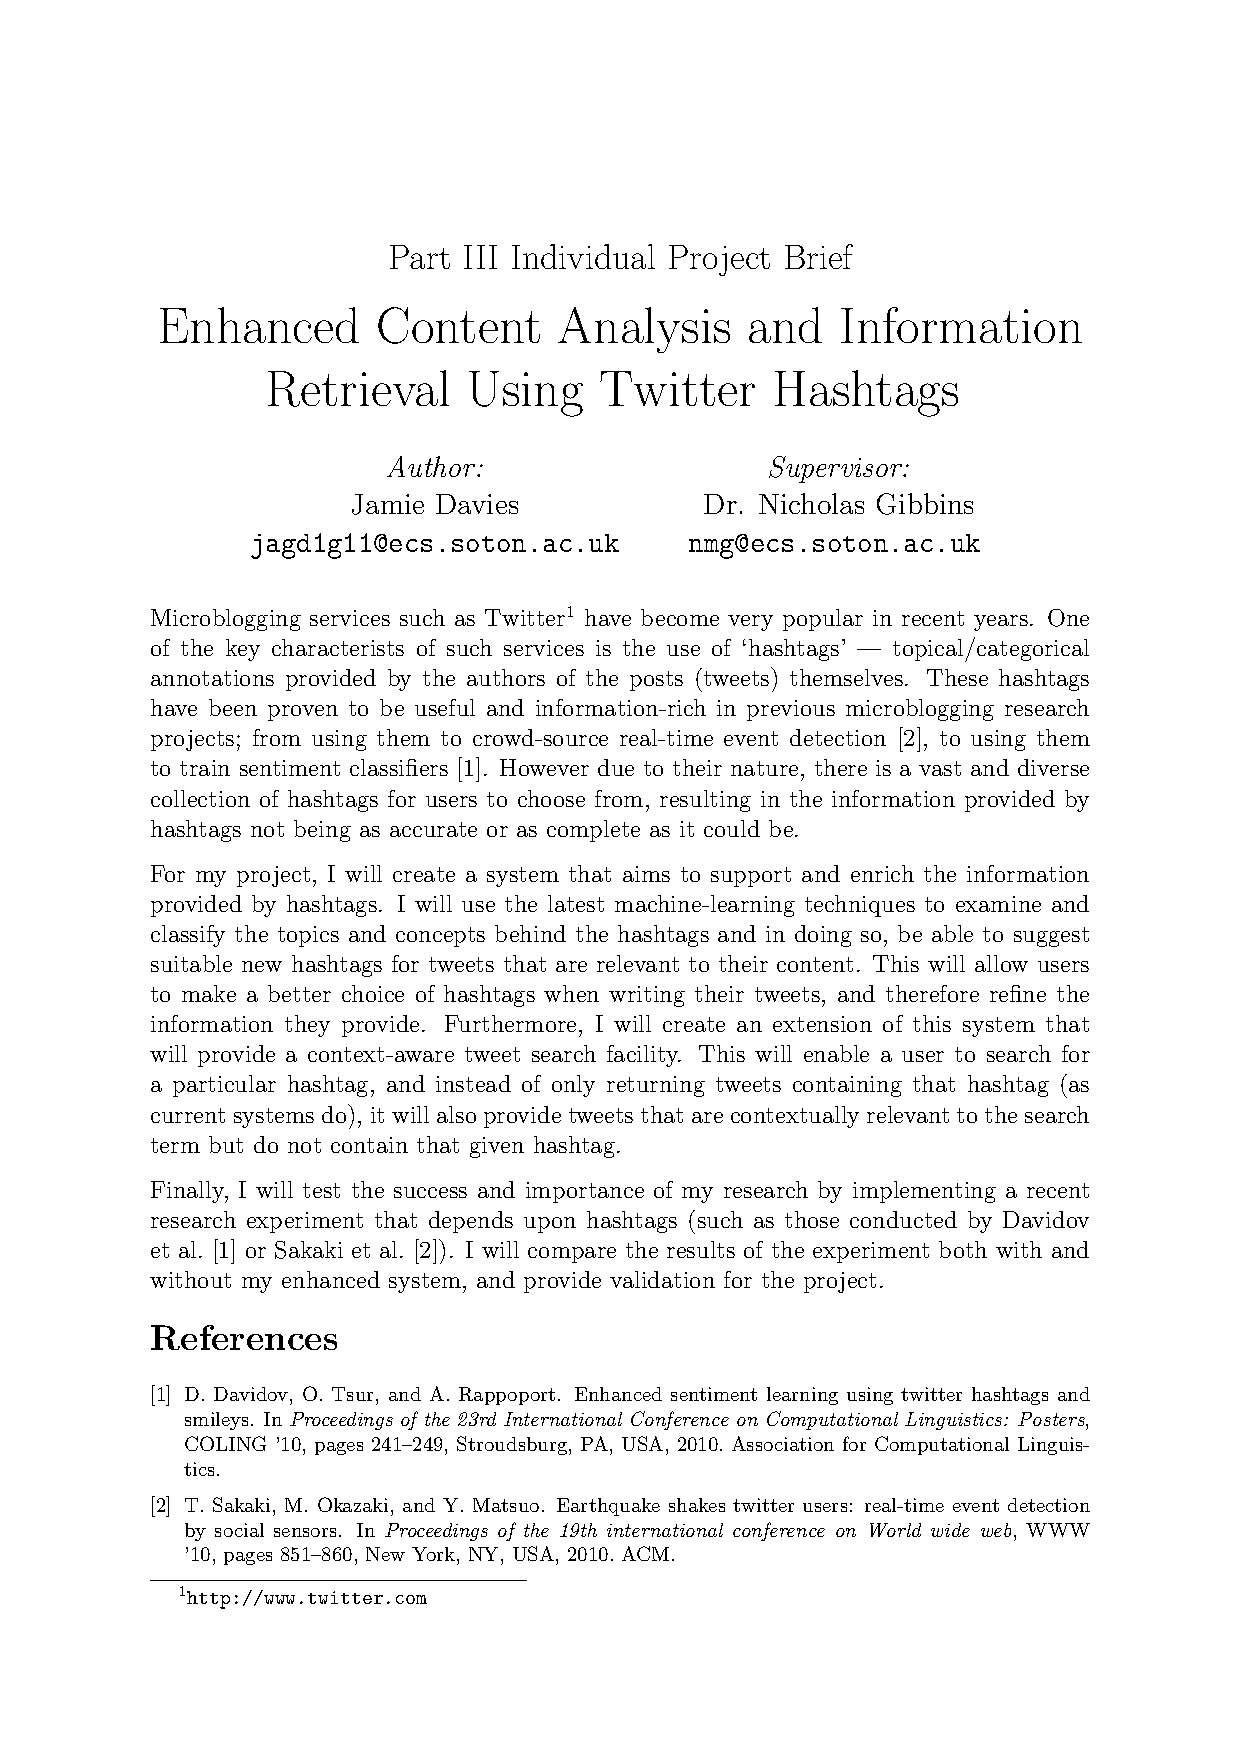
\includegraphics[scale=0.9]{../brief/brief.pdf}
\end{appendices}
\pagebreak

\setcounter{secnumdepth}{0}
\chapter{References}
{\footnotesize \printbibliography[heading=none]}

\end{document}
